\chapter{Simulation, data processing, and event reconstruction}\label{chap:reco}
\minitoc
The data sets, based on the proton-proton (pp) collisions recorded with the CMS detector, are centrally provided in the \texttt{MINIAOD} format~\cite{MiniAOD}. This format contains only parts of the original event and detector information relevant for most of the physics analyses. An analysis looking for deviations from expectations from the SM is supposed not to be biased while development. Thus, SM and signal simulations are performed, and are centrally provided by the CMS collaboration. These are also provided in the \texttt{MINIAOD} format with extended generator information.\\
All available data sets, including measured data and simulation, are further processed with the help of the CMS software framework (CMSSW\footnote{Version 8.0.26})~\cite{CMSSW}, the CMS Remote Analysis Builder (CRAB3)~\cite{CRAB}, and the resources of the Worldwide LHC Computing Grid (WLCG)~\cite{Grid}, to obtain files with significantly reduced size. The obtained reduced information is stored in the \texttt{ROOT}~\cite{ROOT} file format, and can be used by analysts with self-developed software~\footnote{Usually composed of parts developed in \texttt{C/C++} and \texttt{Python}}.\\
\\
In this chapter, at first the used data samples are introduced. Thereafter, an overview of simulation is given, while the simulated samples used in this analysis are reviewed. After that, the event reconstruction performed on all data sets is explained. A more detailed view is given on the reconstruction and identification of physics objects.\\

Protons are objects composed of many different quarks and gluons. The probability to find a distinct parton of a proton with a specific momentum in a deep-inelastic-scattering is given by parton distribution functions (PDFs)\cite{PDF}, that need to be extracted from fits to data, since they are not predicted by QFT.
% Hence, an event measured with the CMS detector is not clean, but shows several effects.
A interaction between two partons of the colliding protons is described in the hard interaction. The products and quantities of these interactions contain the most interesting physical information. Due to the structure of protons, many different lower energy particles can be produced in interactions between additional partons (multi-parton-interactions). These remnants of the scattering process, together with reconstructed remnants of the protons, are denoted as the underlying event. More important for proton-proton colliders is pileup,which denotes interactions between additional protons in the same bunch crossing as the hard interaction.

\section{Data sets}\label{sec:datasets}
This analysis uses different data sets based on the pp-collisions of the LHC with a center-of-mass energy of $13\TeV$ in 2016 and recorded with the CMS detector, corresponding to an integrated luminosity of $35.9\fbinv$. Each primary data set (PD) is a composition of events recorded with similar HLT trigger paths. The \texttt{DoubleMuon} and \texttt{DoubleEG} PDs are used in the central part of the analysis for the signal selection, since they contain events with at least two muons or electrons, respectively. \texttt{MET} and \texttt{HT} PDs are used for trigger efficiency measurements, and the \texttt{MuonEG} PD is used to extract a selection relevant for the background prediction. For a list of used triggers see \refSec{sec:triggEff}.\\
The different PDs are separated into several single samples for different run eras throughout 2016.
% The paths of the used samples, available via the CMS data set bookkeeping service (DBS)~\cite{DASBookkeeping}, with the \texttt{03Feb2017} version of reconstruction are listed in \refTab{tab:datasets}.
The paths of the used samples, available via the CMS data set bookkeeping service (DBS)~\cite{DASBookkeeping} are listed in \refTab{tab:app_datasets} in the additional material.




\section{Simulation}\label{sec:Simulation}
The simulation process for SM background and SUSY signal samples can be divided into three major steps, which are very similar for both cases. At first, for a specific process events are simulated with an event generator. The event generators used for the generation of the samples considered in this analysis are \MADGRAPH5 in leading order (LO) configuration~\cite{Madgraph1,Madgraph2,Madgraph3}, \MADANDMC in next-to-leading order (NLO)~\cite{Madgraph1,AMCATNLO}, \PYTHIA~\cite{Pythia} for both cases of accuracy, or \POWHEG~\cite{Powheg1,Powheg2}. Matrix elements for the contributing diagrams are computed, and via convolving with PDFs, cross sections are calculated. These cross sections later can be used to rescale the simulation event yield to a given integrated luminosity. Thus, the simulation can be performed with much higher statistics than data in order to minimize the statistical uncertainty of the simulation.\\
Depending on the choice of the chosen generator, a separate generator for the simulation of hadronic showers must be used. This is done with \PYTHIA. A matching with the \textsc{MLM}~\cite{Madgraph2} (LO) or \textsc{FXFX}~\cite{AMCATNLO} (NLO) matching schemes is performed, so that partons generated in matrix element calculations corresponding to the hard interaction, and partons generated with \PYTHIA in the showering for, \eg, initial state radiation (ISR), are not double counted. The hadronization of the partons (quarks and gluons) is simulated also with \PYTHIA, based on the confinement of color charged particles.  This, together with the underlying event and pileup, is all covered by the \textsc{CUETP8M1} generator tune~\cite{Tune}. It is based on $7\TeV$ proton-proton CMS and proton-antiproton CDF measurements. The PDFs used for the generation of the MC samples are provided by the \textsc{NNPDF} 3.0 sets~\cite{NNPDF}.\\
The big next step, which is the most time and resource consuming part, is the simulation of the detector response. A full model of the CMS detector was constructed with the \GEANTfour~\cite{Geant} package. Hence, it allows a precise simulation of the detector response for the events generated with the procedure described above. In the \GEANTfour package, material and particle properties, detector effects, and decay structures are considered in the simulation process. Since this procedure is very time consuming, but leads to a high accuracy, a different method is chosen for signal processes. For the generation of SUSY samples, where theoretical uncertainties dominate and events for many different signal points for each model need to be generated, the CMS \textsc{FASTSIM} package is used~\cite{FastSim}. It is based on a simplified geometry and parametrizations, yielding a reduction in runtime of the factor $\approx100$. If the "FullSim" and "FastSim" performances are compared~\cite{FastSimQuality}, a agreement within $\approx10\%$ for all distributions, such as momenta of particles or jet multiplicity, is observed.\\
\\
All simulated processes used in this analysis are listed in \refTab{tab:MCsamples} together with their corresponding cross sections used to rescale the samples later on. The DBS paths are given in the appendix in \refTab{tab:app_MCsets}.\\

\begin{table}[htb]
 \centering
 \caption{All SM simulated samples used in the analysis with their cross sections. For their corresponding accuracy refer to the text. Additional k-factors to obtain NNLO cross sections for the $\PZ\PZ$ samples are applied per event in dependence of the $\pt$ of the diboson system. All samples are of the \texttt{MINIAODSIM} format.}
 % \scriptsize
 \label{tab:MCsamples}
 \begin{tabular}[width=\textwidth]{ll|ll}
  \hline
  \normalsize{process}                             & \normalsize{$\sigma\,[\mathrm{pb}]$} & \normalsize{process}                         & \normalsize{$\sigma\,[\mathrm{pb}]$} \\\hline
  \scriptsize{\textbf{ttbar}}                      &                                      & \scriptsize{\textbf{diboson}}                &                                      \\
  $\ttbar\to\ell^{+}\PGn\cPqb+\ell^{-}\PAGn\cPaqb$ & $87.31$                              & $\PZ\PGg\to2\ell\PGg$ ($\pt^{\PGg}<130\GeV$) & $124.936$                            \\
  \scriptsize{\textbf{ttbarGamma}}                 &                                      & $\PZ\PGg\to2\ell\PGg$ ($\pt^{\PGg}>130\GeV$) & $0.1488$                             \\
  $\ttbar\PGg\to2\ell2\PGn2\cPqb\PGg$              & $1.679$                              & $\PW\PZ$                                     & $4.9125$                             \\
  $\ttbar\PGg\to4\PQq2\cPqb\PGg$                   & $3.482$                              & $\PZ\PZ\to2\ell2\PGn$                        & $0.5644\cdot k(\pt^{ZZ})$            \\
  $\ttbar\PGg\to\ell\PGn2\cPqb2\PQq\PGg$           & $2.509$                              & $\PW\PW\to2\ell2\PGn$                        & $12.178$                             \\
  \scriptsize{\textbf{DrellYan}}                   &                                      & $\PW\Pg\to\ell\PGn\PGg$                      & $489$                                \\
  $\PZ/\PGg^{*}\to2\ell$                           & $5765.4$                             & \textbf{W jets}                              &                                      \\
  \textbf{single top}                              &                                      & $\PW+jets$                                   & $61526.7$                            \\
  $\PWp\to\cPqt\cPaqb$                             & $3.36$                               & \textbf{triboson}                            &                                      \\
  $\cPq\cPaqb\to\cPq^{'}\cPaqt$                    & $80.95$                              & $\PW\PW\PGg$                                 & $0.2147$                             \\
  $\cPq\cPqb\to\cPq^{'}\cPqt$                      & $136.02$                             & $\PW\PZ\PGg$                                 & $0.04123$                            \\
  $\cPaqb\to\PWp\cPaqt$                            & $11.7$                               &                                              &                                      \\
  $\cPqb\to\PWm\cPqt$                              & $11.7$                               &                                              &                                      \\
  \hline
 \end{tabular}
\end{table}



The Drell-Yan (DY) $\PZ/\PGg$ process, as well as the diboson $\PZ\PGg$ and $\PW\PGg$ processes, and triboson production of $\PW\PW\PGg$ and $\PW\PZ\PGg$ are generated with \MADANDMC with NLO accuracy. Top pair production in association with a photon ($\ttbar\PGg$) and the production of a $\PW$ boson in association with jets are also simulated using the \MADANDMC generator with NLO accuracy. Top pair production with leptonic decays ($\ttbar\to 2\ell 2\PGn 2\cPqb$), diboson production of $\PW\PZ$, $\PZ\PZ$, $\PW\PW$, and all single top production processes are generated using \POWHEG.
Diboson $\PW\PW$ and $\PW\PGg$ production, $\PW+jets$ production, triboson $\PW\PW\PGg$ and $\PW\PZ\PGg$ production, and all single top production channels are grouped together and denoted as "other" in the following.
Cross sections calculated with NLO and next-to-next-to-leading order (NNLO) accuracy~\cite{xsec1,xsec2,xsec3,xsec4,xsec5,xsec6,xsec7,xsec8,xsec9} are used for the normalization of the samples.\\
The generator used for the signal simulation production is \MADGRAPH\_\MCATNLO for the simplified models, and \PYTHIA8 for the full GGM model. The corresponding DBS paths are also listed in the appendix in \refTab{tab:app_signalsets}.
The cross sections used in the signal normalization are calculated at NLO accuracy for the full GGM scenario, and at NLO+next-to-leading logarithmic (NLL) accuracy for the two simplified models~\cite{sxsec1,sxsec2,sxsec3,sxsec4,sxsec5,sxsec6,sxsec7,sxsec8,sxsec9}.
For the electroweak SMS, the applied cross sections are calculated for the $\charginoOne\neutralinoOne$ and $\charginoOne\charginoOneBar$ production channels with squarks and gluinos decoupled, and the sum of both is used. In the cross section calculations of gluino pair production for the other SMS, squark decoupling is assumed. The applied cross sections for the GGM scenario are obtained using a full model, thus being different from the ones used for the electroweak SMS.\\
For the GGM model, signal points are generated with wino masses ranging from $215\GeV$ to $1015\GeV$, and bino masses ranging from $205\GeV$ to $m(\widetilde{W})-10\GeV$ in intervals of $25\GeV$.
In case of the \texttt{TChiZG} SMS, points are generated with NLSP masses in the range of $300-1300\GeV$ in steps of $25\GeV$. The grid of points generated for the \texttt{T5bbbbZG} strong production SMS includes gluino masses in the range of $800\GeV$ to $2500\GeV$, while the NLSP mass range is scanned from $10\GeV$ to $m(NLSP)=m(\widetilde{g})-10\GeV$ in non equidistant steps.\\
\\
As mentioned above, the number of generated events $N_{Gen}$ is very high. Thus, with the measured integrated luminosity $\Lumi$  and a given cross section $\sigma$, a global event weight of
\begin{equation}
 w = \frac{\Lumi \cdot \sigma}{N_{Gen}}
\end{equation}
is used to rescale the simulation to the physical expectation.\\
Additional event weights are applied on the simulation to account for differences in the pileup distribution between data and simulation. To improve on the \MADGRAPH modeling of the multiplicity of additional jets arising from initial state radiation, SUSY SMS events are reweighted as a function of $N^{ISR}_{Jet}$ or the transverse momentum of the ISR system, to improve the agreement with observations in data.
The latter is based on studies of the transverse momentum of $\PZ$ events.~\cite{NISRweight}.
The differences to unity for the reweighting factors are considered as systematic uncertainties later on.
The \POWHEG \ttbar simulation is also reweighted as a function of the transverse momentum of the top system, based on studies in top pair production cross section measurements~\cite{topWeight1,topWeight2,topWeight3,topWeight4} to improve the agreement of the transverse momentum of the top quark with data.

\subsection*{Overlap removal}\label{sec:overlap}

Because a very special phase space region is investigated in this analysis, effects play a role, where different physical processes described in higher orders lead to a redundant modeling of distinct diagrams in the matrix element calculation. For each of these processes distinct simulated samples are available, and multiple ones will be used in order to achieve a precise modeling of the phase space region of interest with low statistical uncertainties. Since these samples are produced for a distinct process only, \eg, $\ttbar$ pair production, NLO contributions in this case overlap with the stand-alone $\ttbar\PGg$ samples, because photon radiation in the initial state on the one hand is an NLO contribution for $\ttbar$ production, but on the other hand also describes $\ttbar\PGg$ production in LO. The same holds for the Drell-Yan $\PZ\PGg^{*}$ process and the NLO $\PZ\PGg$ diboson production. To avoid double counting of events, these overlaps need to be removed.\\
Therefore, the MC simulation for those processes was studied on generator level, to understand which event signatures are exactly produced in both samples. Events that have a signature like in samples where photons are produced in the LO matrix element calculations, are removed from the inclusive samples, to achieve a common higher order description of the selected phase space. Since different generators are used to simulate the different processes, different strategy to remove the overlaps were studied, to ensure that all samples can be used without concerns, and double counting of diagram contributions is rejected.


\section{Event and particle reconstruction and identification}\label{sec:reco}
To maintain both a precise and robust particle reconstruction, and flexibility in the identification of physical objects, such as electrons or photons, based on the global reconstruction, particle reconstruction and identification is divided in two major parts. This is needed, since different types of analyses, such as searches or SM precision measurements have different needs for the requirements of their selected particles in terms of efficiency, misidentification, and resolution.\\
In the global event reconstruction, at first, particles and their properties, such as momentum, energy, and trajectory, are reconstructed with the Particle Flow (PF) algorithm~\cite{ParticleFlow} by combining information from all CMS subdetectors. After that, identification criteria determined by specialized CMS physics objects groups (POGs) are applied, dependent on the choice of the analyst regarding the demands mentioned above.\\
In the following the PF algorithm is briefly introduced by explaining its main features, whereafter more detailed definitions of the physical objects are given.

\subsection{Particle flow}
Traditionally, particles in multi-purpose high energy detectors are identified by their information collected in a certain subdetector component. Electrons for example are identified by measuring the deposited energy in the ECAL, and jets consisting of neutral and charged hadrons and photons are measured independently from informations of the tracker and the muon chambers just with the help of the measurements of the calorimeters. To compensate the only sufficient HCAL performance of the CMS detector, a different method is applied, where all information of all subdetectors are combined and global particle elements are identified. Thus, the excellent performance of the CMS tracking system, the high granularity of the ECAL, and the highly efficient muon tracking system can be exploited. This yields the basis of the particle flow event reconstruction, which showed great performance for the first time in its application in the CMS experiment.\\
The PF reconstruction and identification procedure is divided in multiple subtasks. Firstly, tracks and clusters are reconstructed separately. Afterwards, they are combined by a linking algorithm. Finally, so-called PF blocks are formed out of the links, and final decisions are made on the type of the particle.\\
A combinatorial track finding algorithm based on Kalman Filtering~\cite{Kalman} is used to reconstruct tracks in three stages. Firstly, seeds are generated that are compatible with tracker hits and therefore with a trajectory of a charged particle. Secondly, trajectories are built by using all tracker layers. Finally, the particle properties, such as momentum and direction, are determined in a fit. The tracking procedure is optimized to maintain a high efficiency by keeping a low misidentification rate. Solely by using this approach, \eg, a tracking efficiency of $99\%$ for muons, and around $70-80\%$ for charged pions is achieved. To further increase the efficiency while retaining the misidentification rate as low as possible, an iterative tracking procedure is realized, where each step has a lower efficiency compared to the approach discussed before, but quality criteria requirements ensure a low misidentification rate.\\
For electrons another separate track reconstruction is realized. In contrast to the tracker based approach described above, an approach based on reconstructed ECAL clusters is used. Thereby, extrapolations back to the inner tracker are realized based on the cluster energy and position,.\\
The muon tracking is also different, since here in addition the muon system can be used to gain further information and increase the efficiency and lower the misidentification rate. Three types of muon tracks are reconstructed. The first are standalone muon tracks, where only information from the muon system, in particular seeds built of hits in the DTs and CSCs, is used to reconstruct a muon trajectory through all muon system subcomponents. Global muon tracks are standalone muon tracks, that can be matched to hits in the inner tracker. Tracker muon tracks are obtained by extrapolating inner tracker tracks to the muon system, and are only considered if at least one muon segment hit matches the extrapolation.\\
The aforementioned clustering algorithm is performed in each subcalorimeter seperately. It is used to measure the energy and direction of neutral particles such as photons and neutral hadrons, and distinguish them from charged hadrons and photons originating from electron bremsstrahlung. Thereafter, a fit based on the assumption of Gaussian-distributed cell entries in topological clusters is realized to obtain the energy and position of each cluster via determination of cluster seeds, where the energy deposits are maximal compared to the neighboring cells.\\
The last important part of the PF based reconstruction is the linking procedure, where all gained information is combined, based on the nature of each particle. Multiple links are then summed up to a particle flow block, in which seperately the final decisions are made. After each identification step, the used subdetector informations, such as tracks and clusters, are removed from the PF block.\\
Muons are identified first, driven by the high reconstruction efficiency and low misidentification rate using the muon system. Except for jet remnants entering the muon system, called punch through, muons are the only particles leaving a signature in the muon system.\\
Electrons and prompt photons are identified next, since they produce very similar signatures in the ECAL due to electromagnetic showers, and also in the tracker, if photons are converted to electron-positron pairs. Finally neutral and charged hadrons, and non prompt photons, \eg, originating from meson decays, are identified.\\
Based on the PF reconstruction, an analysis-specific physical object selection can be performed on top of the PF objects, which will be discussed in the following.
















% Particles are reconstructed and categorized by PF in five classes, namely muons, electrons, photons, and both neutral and charged hadrons. The decisions are made based on two major reconstruction steps, finding and reconstructing tracks of charged particles, and separate clustering of ECAL and HCAL entries, to reconstruct the energy deposit of the particles' showers.\\
% The track finding algorithm based on Kalman filtering~\cite{Kalman} iteratively generates seeds for the tracks, builds trajectories, and performs a final fit to determine the particle properties, such as direction and momentum based on information of the inner tracker.
% For particles such as muons and electrons, additional tracking algorithms are used to determine a more accurate description of the particle's properties. For muons, additional information of the muon system is used to directly classify three types of non exclusive muon tracks. Standalone muon tracks are reconstructed using only informations of the muon system. If inner tracker tracks can be matched to entries in the muon system, they are called tracker muon track. And in cases where muon system tracks are matched to inner tracks, these are called global muon tracks.
% For electrons additional fitting procedures combining tracker and ECAL informations are used to cope the characteristics of the electromagnetic showers~\cite{GSFTrack}. Therefore, superclusters are built within the ECAL by combining nearby clusters, and the seeds determined with the tracker based approach described above, together with this ECAL based reconstructed seeds, are used in a common track fit.\\
% The clustering algorithm for the ECAL and HCAL also determines cluster seeds at first based on local energy maxima, and afterwards adds cluster entries fulfilling certain energy criteria to obtain topological clusters.\\
% The following combination and linking of the determined information is motivated by the main characteristics of the particle interactions:\\
% Photons are neutral particles, and therefore leave no track in the detector, but only interact electromagnetic. Thus, they are stopped in the ECAL by generating electromagnetic showers. They can also undergo electron-positron pair production, resulting also in electromagnetic showers in the ECAL.\\
% Electrons are charged particles. Hence, their tracks are reconstructable in the tracker, and the energy deposit happens also via electromagnetic shower generation due to Bremsstrahlung in the ECAL. Accordingly, electrons and photons are very similar objects in the reconstruction procedure.\\
% Muons are mainly identified by the informations of the muon system, since no other particles except for very high energetic jets punching through the solenoid and outer HCAL, are capable of reaching the muon chambers. By combining the inner tracks with the entries of the muon chambers, a clear and precise muon identification is maintained.\\
% Charged and neutral hadrons are reconstructed by clusters in the HCAL, and can be differentiated by corresponding matching tracks in the tracker. Parts of non-prompt photons, \eg coming from meson decays, are also reconstructed as neutral hadrons.\\
% The order of particle reconstruction is based on the accuracy and precision of the available information. Thus, muons are identified first, followed by electrons and prompt photons. After that, neutral and charged hadrons, and non-prompt photons are identified.\\
% All these informations obtained by the PF algorithm provide the basis for the final physical object identification applied by the analysts.

\subsection{Primary vertex}
The primary vertex of an event is defined by the vertex with the largest sum of associated transverse momenta squared determined by vertex reconstruction algorithms~\cite{vertex}, and needs to be reconstructed within a distance of $24\cm$ in z direction, and $2\cm$ in the x-y-plane.


\subsection{Muons}
Muons are required to have a transverse momentum larger than $15\GeV$. Because the muon chambers extend only to a pseudorapidity range of $|\eta|<2.4$, muons need to be reconstructed within this region. In addition, muons have to pass quality requirements suggested by the CMS collaboration, yielding a $\approx 98\%$ efficiency~\cite{MuonIDPerf}.\\
A muon candidate needs to be reconstructed as a PF muon, and either as a global muon or a tracker muon. If it is reconstructed as a global and a as tracker muon, the segment compatibility, which is a measure for the comparability between the tracker tracks and an extrapolation to the muon system, has to be larger than $0.303$. In addition, more than $80\%$ of the inner track layers need to be used in the track fit, the normalized goodness of fit ($\chi^2/ndof$) needs to be less than $3$, the match between the standalone muon position and the tracker muon must have $\chi^2<12$, and the maximum $\chi^2$ found by a kink finding algorithm, which tries to separate the track into two independent tracks, needs to be smaller than $20$. If the muon is reconstructed exclusively as a tracker muon, only the segment compatibility needs to be greater than $0.451$, and the other requirements on the track quality are removed.\\
Besides the identification requirements, conditions on the position of the track relative to the reconstructed primary vertex are imposed. In the transverse direction ($d_{xy}$), muon tracks need to be closer than $0.05\cm$ to the vertex, and in the longitudinal direction ($d_z$), the distance needs to be smaller than $0.1\cm$. To quantify the dominance of an object with respect to is surrounding particles in its vicinity, the concept of isolation is introduced. A cone dependent isolation is used, called mini isolation, where the cone size in the $\phi-\eta$ plane is calculated relative to the transverse momentum of the particle as follows:
\begin{equation}
 R = \text{max}\left(0.05,\text{min}\left(0.2,\frac{10\GeV}{\pt}\right)\right).
\end{equation}
Pileup corrections are also taken into account in the mini isolation calculation.
The determined energy deposited in the cone around the muon must not exceed $10\%$ of the transverse momentum of the particle.


\begin{table}[h!]
 \centering
 \caption{Identification criteria for muons, spread for muons being reconstructed as solely tracker and as tracker and global muons.}
 \label{tab:muonID}
 \begin{tabular}{lcc}
  Variable                                            & \multicolumn{2}{c}{Value}                     \\\hline
                                                      & tracker and global muon        & tracker muon \\\hline
  segment compatibility                               & $>0.303$                       & $>0.451$     \\
  fraction of valid inner tracker hits                & $>0.8$                         & -            \\
  normalized $\chi^2$ of global track fit             & $<3$                           & -            \\
  chi2localposition (track standalone position match) & $<12$                          & -            \\
  kink finder                                         & $<20$                          & -            \\\hline
  $\pt$                                               & \multicolumn{2}{c}{$>15\GeV$}                 \\
  $\eta$                                              & \multicolumn{2}{c}{$<2.4$}                    \\
  mini isolation                                      & \multicolumn{2}{c}{$<0.1$}                    \\
  $d_{xy}$                                            & \multicolumn{2}{c}{$<0.05\cm$}                \\
  $d_z$                                               & \multicolumn{2}{c}{$<0.1\cm$}                 \\\hline
 \end{tabular}
\end{table}

% \begin{table}[tbp]
%  \label{tab:muonID}
%  \centering
%  \begin{tabular}{lll}
%   Variable                                            & Value      \\\hline
%   reconstructed as tracker muon                       & true       \\
%   fraction of valid inner tracker hits                & $>0.8$     \\
%   normalized $\chi^2$ of global track fit             & $<3$       \\
%   chi2localposition (track standalone position match) & $<12$      \\
%   kink finder                                         & $<20$      \\
%   segment compatibility                               & $>0.303$   \\\hline
%   segment compatibility                               & $>0.451$   \\\hline
%   $\pt$                                               & $>15\GeV$  \\
%   $\eta$                                              & $<2.4$     \\
%   miniIsolation                                       & $<0.1$     \\
%   $d_{xy}$                                            & $<0.05\cm$ \\
%   $d_z$                                               & $<0.1\cm$
%  \end{tabular}
% \end{table}



\subsection{Electrons}
The list of requirements imposed on the electron selection is driven by a symmetric approach between the two lepton selections. The same conditions on the distance to the primary vertex, ($d_{xy}<0.05$, $d_z<0.1$), pseudorapidity ($|\eta|<2.4$), and transverse momentum ($\pt>15\GeV$) need to be fulfilled. The mini isolation criterion is relaxed to $20\%$.\\
The identification requirements determined by the CMS Collaboration~\cite{ElectronID} separately for electrons reconstructed in the ECAL barrel (EB: $|\eta_{Supercluster}|<1.479$) and endcap (EE: $|\eta_{Supercluster}|>1.479$) region are listed in \refTab{tab:eleID}.
\begin{table}[tbp]
 \centering
 \caption{Identification criteria for electrons given separately for reconstructed electrons in the barrel and endcap.}
 \label{tab:eleID}
 \begin{tabular}{lcc}
  Variable                       & \multicolumn{2}{c}{Value}                   \\\hline
                                 & EB                             & EE         \\\hline
  $\sigma_{i\eta i\eta}$         & $<0.00988$                     & $<0.0298$  \\
  $\Delta\eta_{Seed}$            & $<0.00311$                     & $<0.00609$ \\
  $\Delta\phi_{In}$              & $<0.00311$                     & $<0.00609$ \\
  $H/E$                          & $<0.253$                       & $0.0878$   \\
  relative combined PF isolation & $<0.0695$                      & $<0.0821$  \\
  $|\frac{1}{E}-\frac{1}{p}|$    & $<0.134$                       & $<0.13$    \\
  \# missing inner hits          & $\leq1$                        & $\leq1$    \\
  Photon conversion veto         & true                           & true       \\\hline
  $\pt$                          & \multicolumn{2}{c}{$>15\GeV$}               \\
  $\eta$                         & \multicolumn{2}{c}{$<2.4$}                  \\
  mini isolation                 & \multicolumn{2}{c}{$<0.2$}                  \\
  $d_{xy}$                       & \multicolumn{2}{c}{$<0.05\cm$}              \\
  $d_z$                          & \multicolumn{2}{c}{$<0.1\cm$}               \\\hline
 \end{tabular}
\end{table}
Here, $\sigma_{i\eta i\eta}$ is a quantity characterizing the width of the electromagnetic shower shape in the ECAL in $\eta$ direction. It is calculated as the weighted variance of energy deposits in the full 5x5 pixel ECAL supercluster. Since jets emerging from hadrons have a wider shower in the ECAL than electrons, a differentiation can be achieved. Consistency between the information of the reconstructed track at the vertex, and the supercluster is required, by setting conditions on $\Delta\eta$, $\Delta\phi$, and the supercluster energy $E$ and track momentum $p$. To further separate electrons from hadrons, more energy should be deposited in the ECAL, rather than in the HCAL ($H/E$). An isolation requirement based on the PF determined isolation, assures that prompt electrons are separated from electrons coming from, \eg, jets. Photons misidentified as electrons are suppressed by imposing a requirement on the number of missing inner hits in the tracker, and an additional veto for photon conversions to electron-positron pairs determined in an $\chi^2$ fit.

\subsection{Photons}
Photons are required to have a transverse momentum larger than $20\GeV$.  Because in the considered SUSY signal scenarios the sparticles typically have high masses, central collisions are needed to produce these in the proton-proton interactions.  Therefore, the sparticles decay mainly in rest, and the photons originating from the decays are produced more centrally im comparison to SM processes. Hence, only photons reconstructed in the ECAL barrel are considered ($|\eta<1.4442|$). Additional identification criteria determined by the CMS Collaboration~\cite{photonID} are listed in \refTab{tab:photonID}.
\begin{table}[h!]
 \centering
 \caption{Identification criteria for photons reconstructed in the ECAL barrel.}
 \label{tab:photonID}
 \begin{tabular}{lc}
  Variable                    & Value                                                \\\hline
  $\sigma_{i\eta i\eta}$      & $<0.01031$                                           \\
  $H/E$                       & $<0.0597$                                            \\
  PF charged hadron isolation & $<1.295$                                             \\
  PF neutral hadron isolation & $<10.910 + 0.0148 \cdot \pt + 0.000017\cdot (\pt)^2$ \\
  PF photon isolation         & $<3.630+0.0047\cdot \pt$                             \\\hline
  $\eta$                      & $<1.4442$                                            \\
  $\pt$                       & $>20\GeV$                                            \\
  \# Pixel Seeds              & 0                                                    \\\hline
 \end{tabular}
\end{table}
Similar to the requirements on $\sigma_{i\eta i\eta}$ and $H/E$ for the electron selection, these conditions in the photon identification ensure the suppression of selecting hadrons faking the photon signature. Additional different isolation criteria lower the amount of selected photons originating from neutral and charged hadrons, and photons created from light meson decays.\\
Requirements on the minimum distance in the $\eta-\phi$ plane between the photon and selected lepton candidates ($\Delta R(\PGg,\ell)>0.3$) significantly reduce contributions from final state radiation (FSR) photons. By requiring that no pixel seed can be assigned to a trajectory between ECAL supercluster and interaction point, a clear differentiation between electrons and photons is achieved.

\subsection{Jets}
Jets are complicated objects due to the complexity of the hadronization and fragmentation processes. Therefore, a sophisticated clustering algorithm is needed to identifiy them and measure their energy properly. Jets are clustered with the anti-$k_T$ algorithm~\cite{AntiKT} included in the \FASTJET package~\cite{FastJet1,FastJet2} with a distance parameter of $R=0.4$. In the clustering procedure, each PF object is considered a pseudojet, and these pseudojets are summed up iteratively until a certain breaking condition is fulfilled. The final jet momentum is defined as the sum of the momenta of the constituents of the jet. Charged hadrons not emerging from the primary vertex are not considered in the clustering. The jet energy is corrected for effects originating from pileup and the detector response, tuned with the help of different data control selections and simulation~\cite{JEC}. Reconstructed jets are required to pass loose identification criteria proposed by the CMS Collaboration~\cite{JetID}, to have a transverse momentum larger than $30\GeV$, and their pseudorapidity must not exceed $|\eta|=3|$. In addition, jets overlapping with photon or lepton candidates in a cone with radius $R=0.4$ in the $\eta-\phi$-plane, are removed from the selection to avoid double counting of objects.


\section{Definition of observables}
Throughout this thesis, different observables are used to define different phase space regions, in particular the signal region and control and validation regions important for the background prediction. All these high level variables are defined based on low level quantities such as the $\pt$ of different objects.


\subsection{Missing transverse momentum}
Missing transverse momentum $\ptmiss$ is one of the most important observables in searches for BSM physics. In typical SUSY models, see \refSec{sec:SUSY}, significant $\ptmiss$ is expected in the events due to the LSP leaving the detector undetected. In SM processes only neutrinos and mismeasurements of, \eg, the jet energies lead to missing transverse momentum, because before a collision the transverse momentum of the colliding protons is nearly negligible. In such SUSY events, the LSP gains a lot of energy in its production in the decays of sparticles with higher masses. Therefore, much more $\ptmiss$ is expected to be produced in SUSY events as in SM processes. Missing transverse momentum quantifies the imbalance of all reconstructed particles in an event and is defined as
\begin{equation}
 \ptmiss= |\ptvecmiss| = |-\sum_{PF objects}\pt_{,i}|.
\end{equation}
Jet energy corrections are propagated to the missing transverse momentum vector to avoid a bias in events with large hadronic activity.

\subsection*{Total hadronic activity $\HT$}
The hadronic activity $\HT$ is defined as the scalar sum of the transverse momenta of all jets, that are clustered with the procedure above, and fulfill $|\eta|<3$ and $\pt>30\GeV$
\begin{equation}
 \HT = \sum_{Jets} |\ptvec_i|.
\end{equation}

\subsection*{Invariant dilepton mass $m_{\ell\ell}$}
The invariant dilepton mass $m_{\ell\ell}$ is defined as the absolute value of the sum of both lepton four momenta
\begin{equation}
 m_{\ell\ell}=|\boldsymbol{p}_{\ell_1}+\boldsymbol{p}_{\ell_2}|.
\end{equation}

\subsection*{The transverse mass $m_{T}$}
If particles decay to invisible and visible objects, the invariant mass of the mother particle cannot be fully reconsructed. In contrast to the calculation of the invariant dilepton mass introduced above, invisible decay products are not measured in the detector. Only the missing transverse energy $\ptmiss$ can be measured, and is only reasonable to be defined in the transverse plain. In such cases, the transverse mass $m_{T}$ of the mother particle can be reconstructed by using only transverse components of all involved fourmomenta.\\
The transverse mass of two objects with transverse momentum $\ptvec^A$ and $\ptvec^B$ yields the transverse mass of the mother particle if both particle emerge from the same decay.
It is defined as
\begin{equation}
 m_T\left(\ptvec^{A},\ptvec^B\right) = \sqrt{2|\ptvec^A||\ptvec^B|\left(1-\cos(\Delta\phi)\right)},
\end{equation}
where $\Delta\phi$ is the angle between $\ptvec^A$ and $\ptvec^B$ in the transverse plane.\\
In cases of one invisible decay product, $m_T$ is calculated assuming that $\ptmiss$ describes the $\pt$ of the invisible decay product. By definition it has an upper limit at the actual mass of the mother particle, and yields therefore good estimate for the total mother particle mass.

\subsection*{The stransverse mass $\mtTwo$}
In case of two identical particles, each decaying to one invisible and one visible particle, the stransverse mass $\mtTwo$~\cite{Mt2_1,Mt2_2} is a useful generalization of $m_T$. In this analysis it is calculated to estimate the mass of the NLSP, which decays to an invisible object, the gravitino, and one visible particle, a Z boson or a photon. It is defined as
\begin{equation}
 \mtTwo = \text{min}_{\ptvec^{\gravitino_1}+\ptvec^{\gravitino_1_2}=\ptvecmiss}\left(\text{max}\left[m_T(\ptvec^{\PZ},\ptvec^{\gravitino_1}),m_T(\ptvec^{\PGg},\ptvec^{\gravitino_1_2})\right]\right),
\end{equation}
where the final value is determined via minimization as indicated by $\text{min}$ in the equation. Descriptively, the algorithm tries to estimate the transverse masses of the mother particles under the assumption, that $\ptmiss$ is composed of exactly one massless particle from  each decay branch.\\
For decays of the NLSP in all signal models, the $\mtTwo$ distribution has a upper limit at the mass of the lightest neutralino, while for all SM backgrounds $\mtTwo$ yields much lower values in comparison to the high SUSY masses. See \refFig{fig:mt2} for a visualization of the described decay structure and a $\mtTwo$ distribution.

\begin{figure}
 \centering
 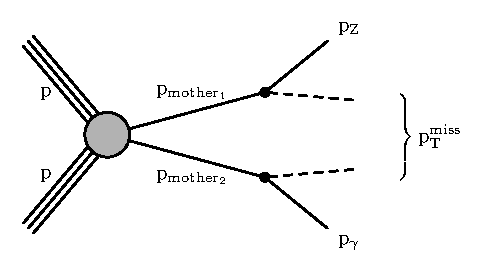
\includegraphics[width=\pairwidth]{figures/mt2/graph}
 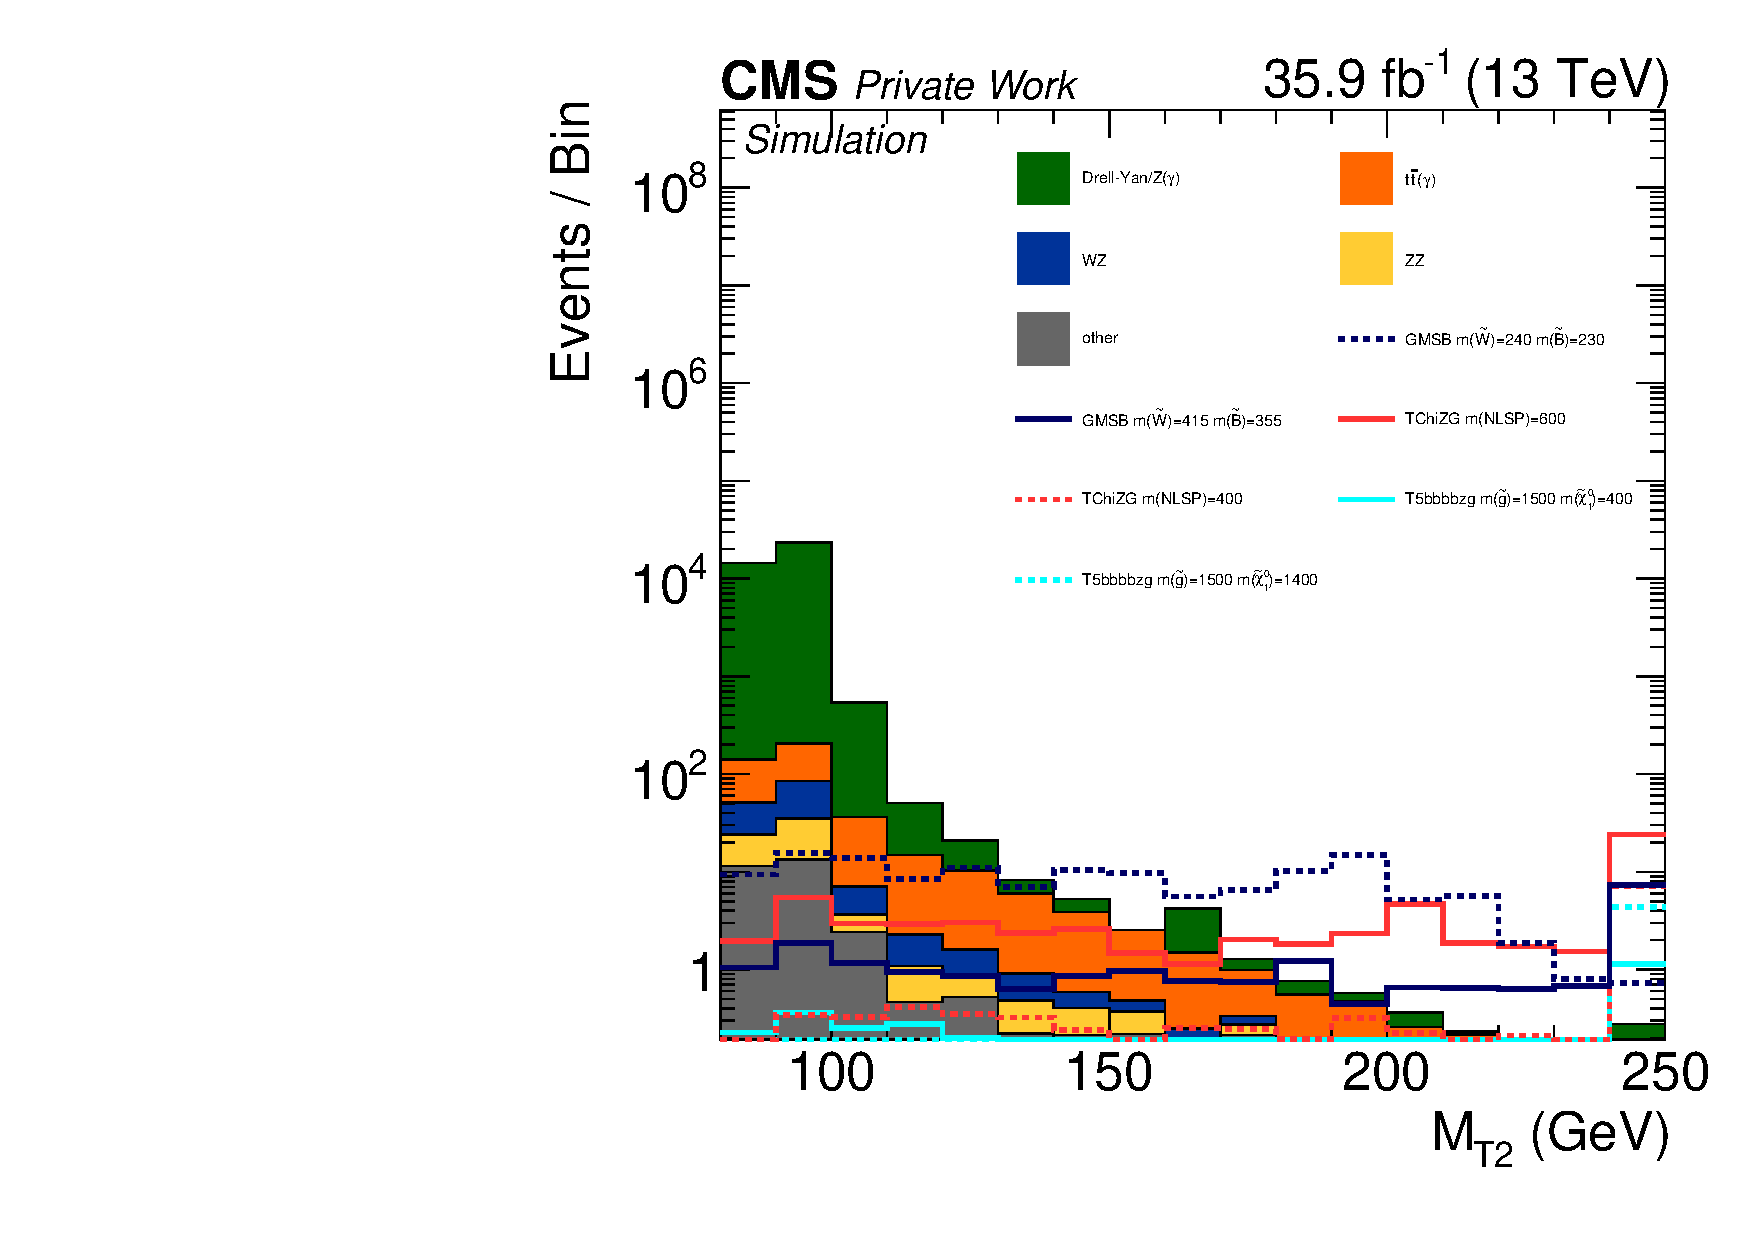
\includegraphics[width=\pairwidth]{figures/plots/onZ_LL_mt2_log}
 \caption{Sketch of decays of pair produced particles to $\ptmiss$ and a $\PZ$ boson or photon respectively (left). Stacked background and different signal points against the stransverse mass $\mtTwo$ (right). Both are obtained from simulation. For each signal model two different signal points are shown. For their masses refer to the legend in the plot.}
 \label{fig:mt2}
\end{figure}


\section{Lepton pair selection and quality requirements}\label{sec:lepPair}
In the analysis, different datasets selected with different dilepton triggers are combined, see \refSec{sec:datasets}. Therefore it is possible, that an event is contained in more than one data set. Hence, it is assured with the following procedure, that no event is double counted. At first, all leptons per event are sorted by their transverse momenta. The leading and subleading\footnote{Called trailing from now on.} lepton are identified. Their flavor combination then determines the classification of the event as "dielectron", "dimuon", or "electron-muon". For instance, a dielectron event is classified as such, if  the event originates from the \texttt{DoubleEG} sample, both the leading and the trailing lepton are electrons, and it is selected by at least one of the dielectron triggers. This set of conditions ensures the exclusivity of the three selections.\\
In addition, there are some requirements imposed on the dilepton system. The trailing and leading lepton need to be separated at least by a distance of $\Delta R=0.1$ in the transverse plane, and the invariant dilepton mass $m_{\ell\ell}$ should be larger than $50\GeV$. The first requirement provides a cleaning between the lepton collections and ensures, that no lepton candidate is counted twice, while the latter threshold is introduced, because the simulation of the Drell-Yan simulation does not include events with lower dilepton masses. Events with lower invariant dilepton masses are not of interest for this analysis, since in the following only leptons originating from a Z boson decay are selected, resulting in an invariant dilepton mass around the Z boson mass of $\approx91\GeV$.\\
Hereafter, the dielectron and dimuon selections are combined to a dilepton selection to increase the statistics in the validation, and especially in the signal region.\\
Additional leptons need to pass the same selection as the trailing lepton.
\\
Also, several event quality filters are applied to reject contaminated events~\cite{MetFilter}.
% \begin{itemize}
%  \item \texttt{HBHE noise filter},
%  \item \texttt{HBHE noise iso filter},
%  \item \texttt{ECAL TP filter},
%  \item \texttt{eeBadSCFilter},
%  \item \texttt{bad PF muon filter},
%  \item \texttt{bad charged hadron filter},
%  \item \texttt{bad muon filter},
%  \item \texttt{beam halo filter}.
% \end{itemize}
The rejected events consist mainly of events with faulty detector signals caused by noise or anomalies, spurious energy deposits in ECAL endcap crystals, cosmic muons, muons being misidentified as charged hadrons, or muons produced in scattering processes with the beam halo.


\section{Used triggers and trigger efficiency measurement}\label{sec:triggEff}
As pointed out in \refSec{sec:datasets}, the events are recorded with various dilepton triggers. For each dilepton combination ($\Pe\Pe,\Pgm\Pgm,\Pe\Pgm$) multiple triggers are used because of the changing instantaneous luminosity over the 2016 run period, and different triggers were active at different times. The main trigger paths are isolated dilepton triggers, while non-isolated trigger paths are added to increase the efficiency for boosted topologies of the dilepton system. A list of all used HLT trigger paths is given in the appendix in \refTab{tab:app_trigger1} and \refTab{tab:app_trigger2}. While the same-flavor dilepton triggers ($\Pe\Pe,\Pgm\Pgm$) are used as signal triggers, the different-flavor triggers ($\Pe\Pgm$) are used to select events needed for the background prediction of the top pair production ($\ttbar(\PGg)$) background. This is explained in more in detail in \refSec{sec:ttbar}. The various dilepton triggers alltogether have transverse momentum thresholds for the dileptons of around $17-33\GeV$ for the leading lepton, and $8-33\GeV$ for the trailing one. Additional triggers with hadronic activity ($\HT$) or $\ptmiss$ thresholds are relevant for the trigger efficiency measurement, which will be presented in the following.
\subsection{Trigger efficiency measurement}
A trigger efficiency curve is characterized by an inefficient part, a more or less sharp transition ("Turn On") to the efficient part, that is ideally located at the nominal threshold of the trigger path, and a flat efficient part.\\
Measuring the trigger efficiency is essential to obtain appropriate transverse momentum requirements for the dilepton system. In the signal simulation using the \textsc{FASTSIM} package no trigger simulation is performed, while it is done for the SM background samples. Therefore, the efficiency needs to be measured also on simulation, such that the signal simulation can be scaled accordingly. In addition, the SM simulation samples will be weighted with a factor, correcting for differences in the efficiency between data and simulation.\\
A logical \texttt{OR} combination of all dilepton triggers with the same-flavor requirements is used. Thus, for an event only one of the used triggers has to be fired to be selected for the key analysis. The combined trigger efficiency $\varepsilon$ is measured using a baseline trigger. An appropriate baseline trigger has to be chosen, meaning that it needs to be uncorrelated to the signal trigger which efficiency is being measured. In addition, the baseline trigger needs to provide a sufficient number of events to ensure a sample of events large enough to reduce the statistical uncertainty of the measurement. The signal trigger efficiency is defined as the number of events passing baseline and signal trigger, divided be the number of events passing only the baseline trigger:
\begin{equation}
 \varepsilon=\frac{\#(baseline \wedge signal)}{baseline}.
\end{equation}
As a consequence, the efficiency of the baseline trigger cancels, and the pure signal trigger efficiency is maintained. As baseline triggers, a combination of various triggers with $\HT$ thresholds is used. These thresholds range from $200-800\GeV$. Therefore, the measurement is not performed on the dilepton data streams, but on the $\HT$ datasets. The event selection consists of the lepton pair selection introduced in \refSec{sec:lepPair} with an additional $\HT>200\GeV$ requirement to ensure, that the baseline triggers are efficient. An additional matching between the selected leptons and the trigger objects responsible for the firing of the triggers is performed.\\
Since dilepton triggers are used, the threshold of the efficient part needs to be determined for each lepton trigger leg seperately. Resulting efficiency curves for all three dilepton combinations measured both on data and simulation are shown in \refFig{fig:triggEff} against the $\pt$ of the trailing lepton. The statistical uncertainties of the individual bins are calculated using $68\%$ confidence level (CL) Clopper-Pearson intervals~\cite{ClopperPearson}. The measurements suffer mainly from the available sample size in the $\HT$ triggered data set, while the available number of simulated events is very high per definition. The electron-muon channel is affected the most by this effect. However, the efficiency curves show the structure of multiple transitions into efficient phases, as it is expected from a combination of triggers with very different ranges of thresholds. As indicated by the dotted lines in the plots, the lepton $\pt$ cut was determined to be $20\GeV$ for the trailing lepton, and $25\GeV$ for the leading one. Although the dielectron and electron-muon triggers are not yet fully efficient at this threshold, as it is the case for the dimuon trigger, this requirement is imposed also on the other two selections in order to obtain a symmetric lepton selection. The mean plateau efficiencies are shown as gray bands with their statistical uncertainties in the plots. The mean efficiency is also measured on simulation, and all efficiency values are given in \refTab{tab:triggEff}. These are obtained by requiring both leptons to pass the $25\GeV$ and $20\GeV$ threshold, respectively. As can be seen, these values do not differ very much from the values quoted in the plots, where no lepton $\pt$ requirement in the selection is imposed. Thus, the leading lepton leg is nearly fully efficient, when the trailing lepton has a $\pt$ larger than $20\GeV$. Additional efficiency values for the same triggers obtained with a $\ptmiss$ baseline selection, that are discussed in the following, are given, too.
The efficiency curves after applying the $\pt$ cuts, are also studied in various other distributions to assure the stability of the used triggers.
\begin{figure}[htb]
 \centering
 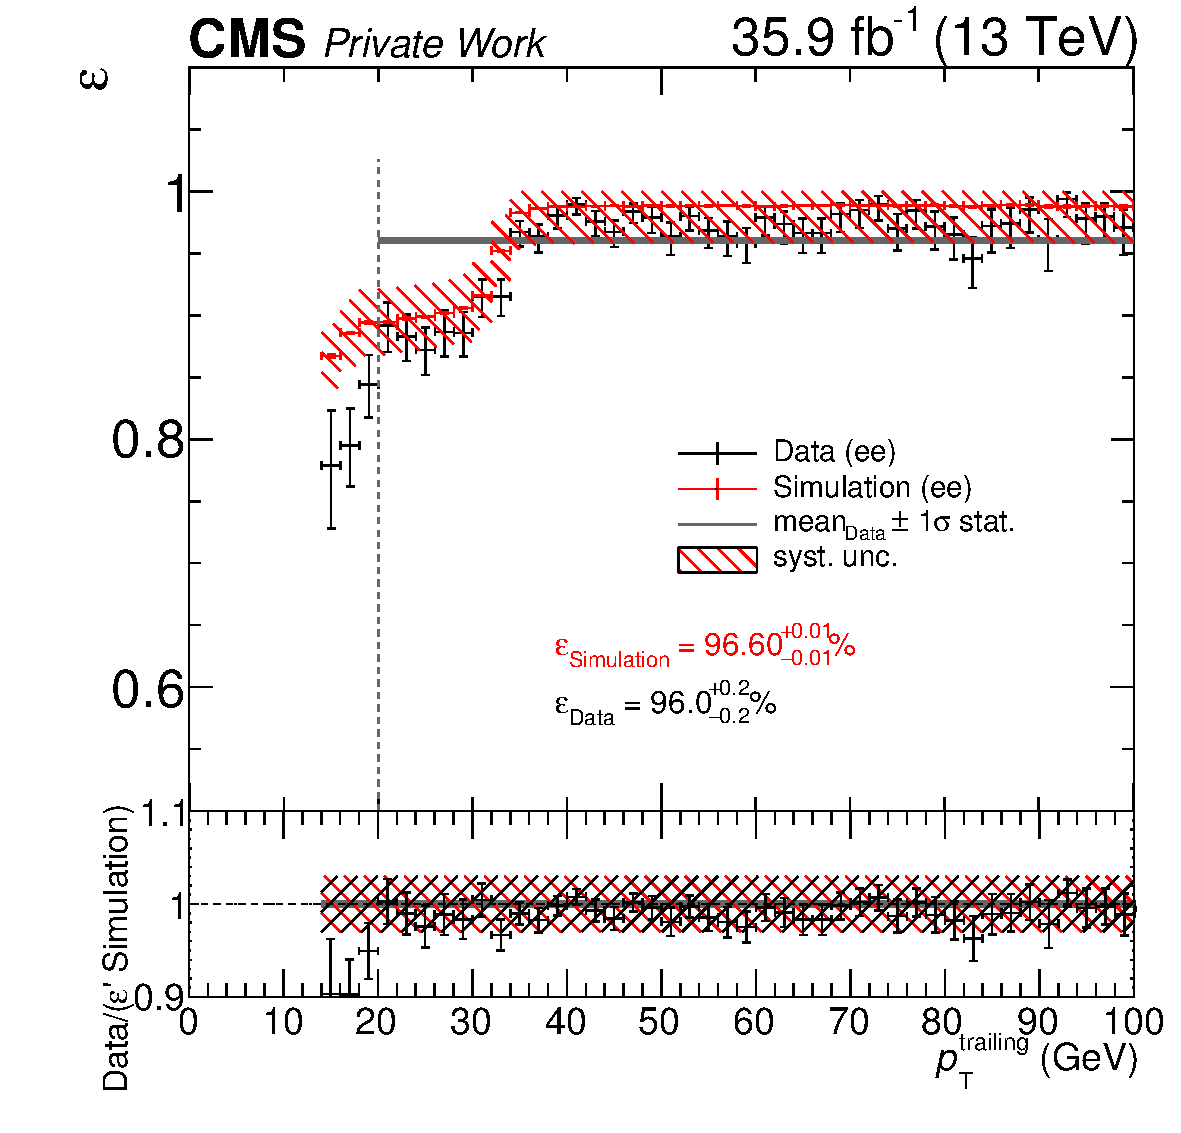
\includegraphics[width=\pairwidth]{figures/triggerStudies/efficiency_dataHT_trigDilep_EE_pt2}
 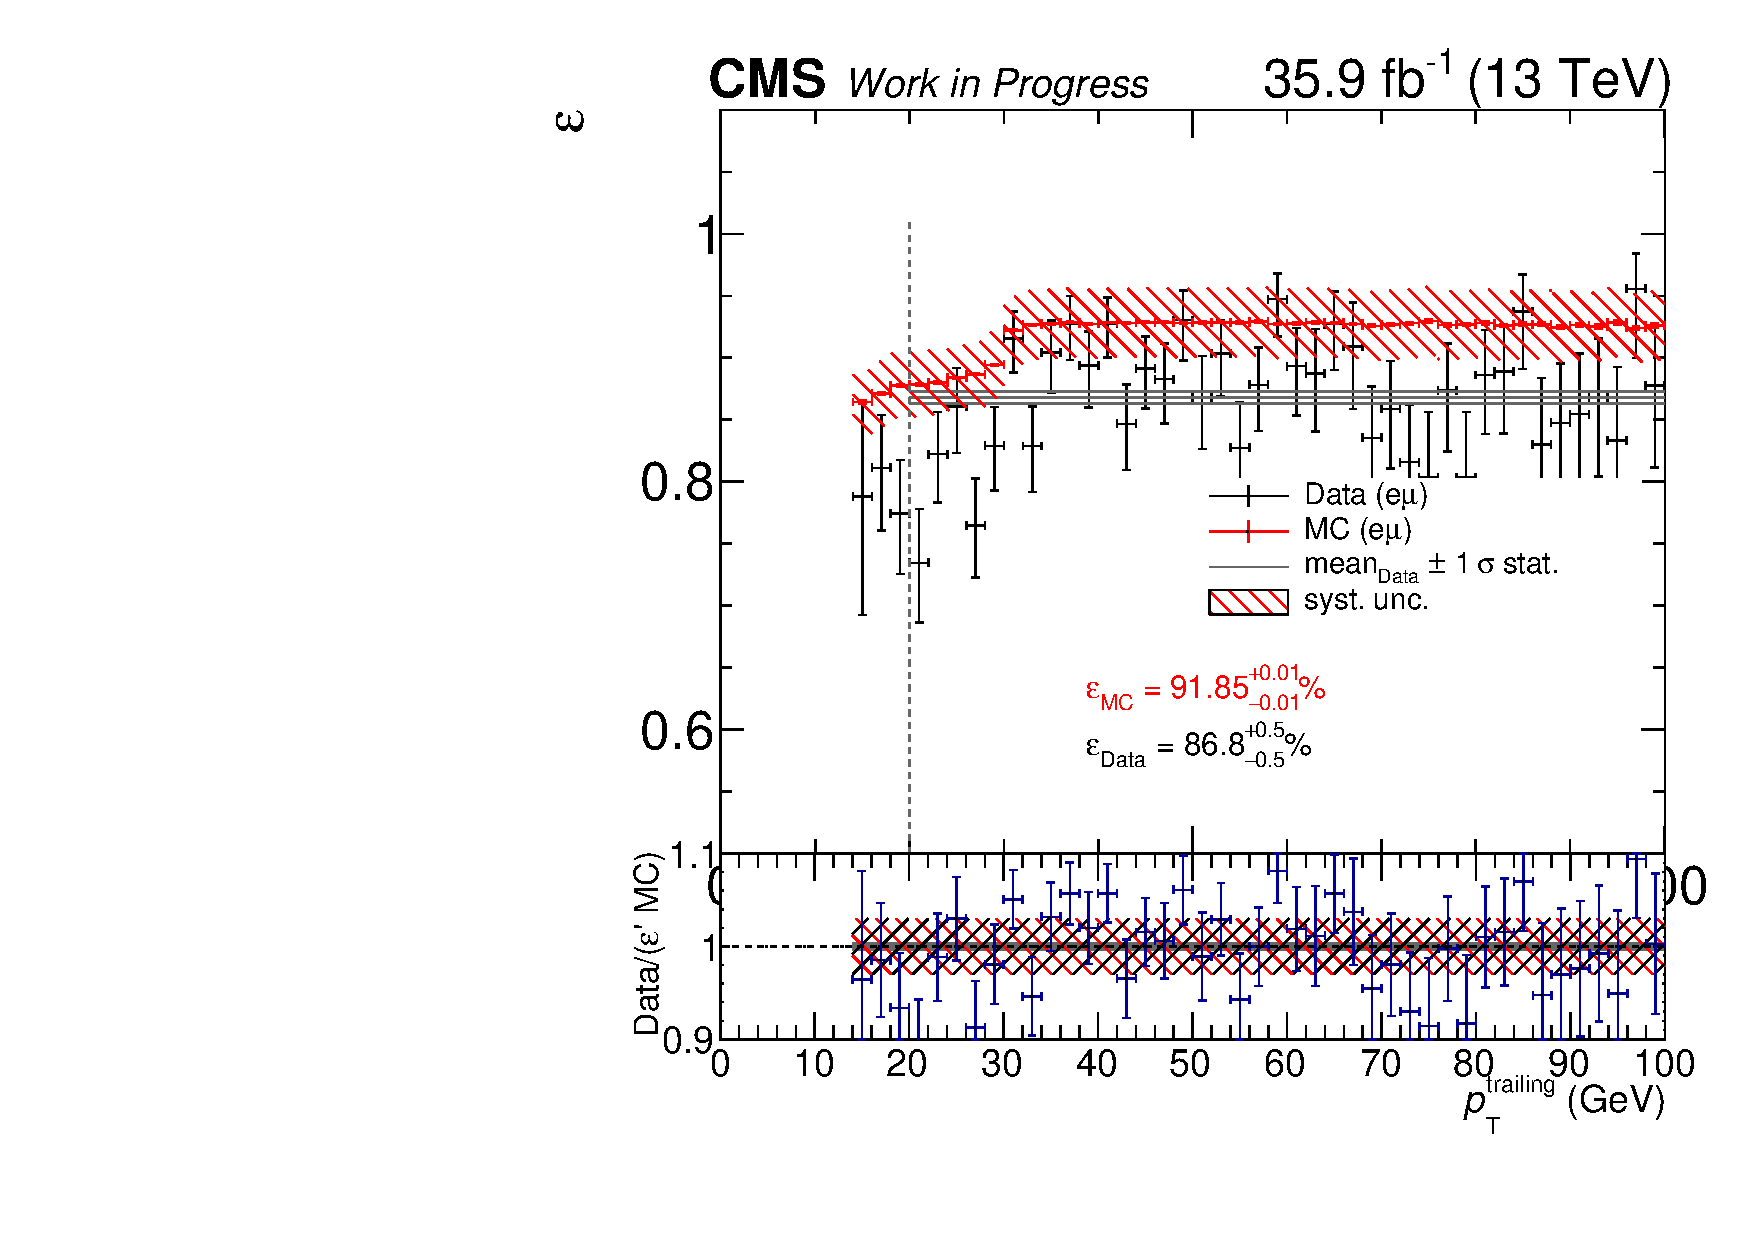
\includegraphics[width=\pairwidth]{figures/triggerStudies/efficiency_dataHT_trigDilep_EM_pt2}
 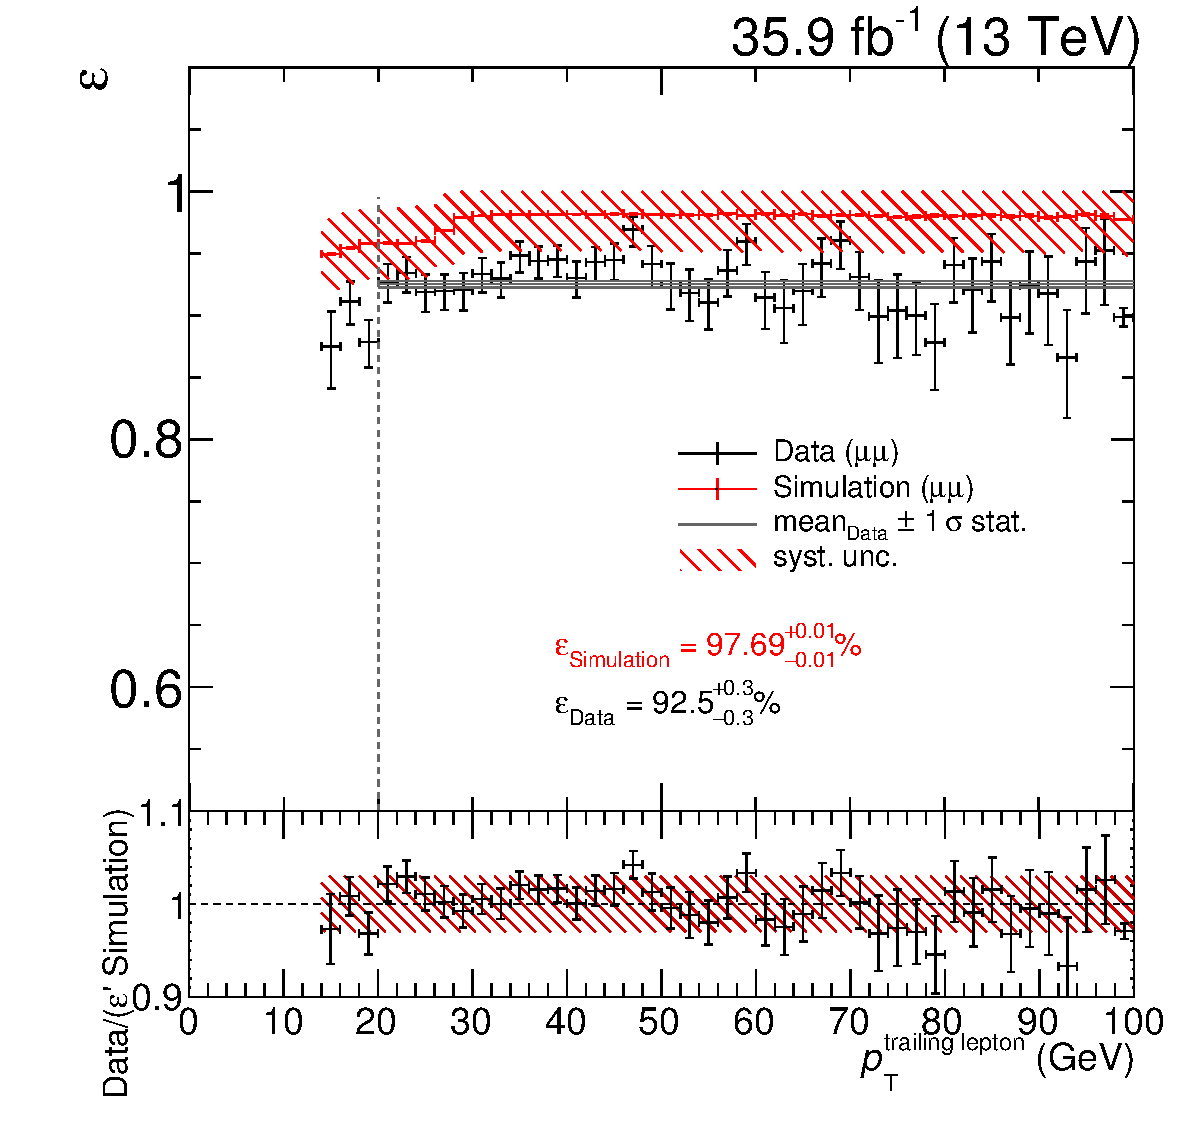
\includegraphics[width=\pairwidth]{figures/triggerStudies/efficiency_dataHT_trigDilep_MM_pt2}
 \caption{Measurement of the combined efficiency for all dilepton trigger combinations on data (black) and simulation (red) for the $\Pe\Pe$ (top left), $\Pe\PGm$ (top right), and $\PGm\PGm$ (bottom) channels. The measurement is performed using various $\HT$ baseline triggers, while the selection consists of the lepton pair preselection, and a $\HT>200\GeV$ requirement. The mean of the data efficiency with its statistical uncertainty (gray band), and the $3\%$ systematic uncertainty on the measurement (red band) are also shown.}
 \label{fig:triggEff}
\end{figure}


\begin{table}[htb]
 \centering
 \caption{Trigger efficiencies determined both on data and simulation for both baseline trigger
  configurations for the $\Pe\Pe$, $\Pe\Pgm$, and $\Pgm\Pgm$ channels.}
 \label{tab:triggEff}
 \begin{tabular}{lllll}
                   & \multicolumn{2}{c}{Data} & \multicolumn{2}{c}{Simulation}                                                         \\\hline
  baseline trigger & $\HT$                    & $\ptmiss$                      & $\HT$                     & $\ptmiss$                 \\\hline
  $\Pe\Pe$         & $96.0^{+0.2}_{-0.2}\%$   & $93.7^{+0.3}_{-0.3}\%$         & $96.60^{+0.01}_{-0.01}\%$ & $96.79^{+0.02}_{-0.02}\%$ \\
  $\Pe\Pgm$        & $86.6^{+0.5}_{-0.5}\%$   & $86.7^{+0.3}_{-0.3}\%$         & $91.85^{+0.01}_{-0.01}\%$ & $91.34^{+0.05}_{-0.05}\%$ \\
  $\Pgm\Pgm$       & $92.5^{+0.3}_{-0.3}\%$   & $93.9^{+0.3}_{-0.3}\%$         & $91.85^{+0.01}_{-0.01}\%$ & $97.62^{+0.02}_{-0.02}\%$ \\\hline
 \end{tabular}
\end{table}


In addition the agreement between rescaled simulation by the factor $\varepsilon'=\varepsilon_{Data}/\varepsilon_{MC}$ and data is shown in the ratio plots beneath the efficiency curves. It can be concluded, that the efficiencies agree within the systematic uncertainty, which is set to cover differences between data and simulation. It is determined to be $3\%$, and is indicated with the red uncertainty band in the plots.\\

As an additional independent check, the whole trigger efficiency measurement was performed also on $\ptmiss$ datasets with $\ptmiss$ baseline triggers, that have thresholds of around $110-600\GeV$. This selected phase space region should be more or less orthogonal the $\HT$ selection. It is also closer to the phase space of the final signal region, since the signal region selection contains a $\ptmiss$ threshold, see \refSec{sec:SRSelection}. Because the efficiency in the low $\HT$ region cannot be studied with the $\HT$ baseline selection due to the inherent inefficiency of these triggers, with the $\ptmiss$ baseline selection this region can be covered. As can be read from \refTab{tab:triggEff}, the values obtained from this method are also in agreement with the efficiencies measured using the $\HT$ selection.\\
Moreover, the pure simulated trigger efficiency was investigated in dependence of $\HT$, to confirm the reliability of the simulation.
